\documentclass[UTF8,a4paper]{ctexart}
\usepackage[margin=1in]{geometry}
\usepackage{threeparttable}
% \usepackage{hyperref}
\usepackage[colorlinks,linkcolor=black,citecolor=black]{hyperref}
\usepackage[section]{placeins}
\usepackage{titlesec}
\usepackage[numbers]{gbt7714}
\usepackage{algorithm}
\usepackage{algpseudocode}
\usepackage{algorithmicx}
\usepackage{amsmath}
\usepackage{float}
\usepackage{array}
\usepackage{graphicx}
\usepackage{subfigure}
\usepackage{fancyhdr}
\usepackage{amssymb}
\usepackage{listings}
\usepackage{color}
\usepackage{bm}
\usepackage{threeparttable}
\usepackage{booktabs}


\floatname{algorithm}{算法}

\definecolor{dkgreen}{rgb}{0,0.6,0}
\definecolor{gray}{rgb}{0.5,0.5,0.5}
\definecolor{mauve}{rgb}{0.58,0,0.82}

\lstset{ %
  language=java,                % the language of the code
  basicstyle=\footnotesize,           % the size of the fonts that are used for the code
  numbers=left,                   % where to put the line-numbers
  numberstyle=\tiny\color{gray},  % the style that is used for the line-numbers
  stepnumber=1,                   % the step between two line-numbers. If it's 1, each line 
                                  % will be numbered
  numbersep=5pt,                  % how far the line-numbers are from the code
  backgroundcolor=\color{white},      % choose the background color. You must add \usepackage{color}
  showspaces=false,               % show spaces adding particular underscores
  showstringspaces=false,         % underline spaces within strings
  showtabs=false,                 % show tabs within strings adding particular underscores
  frame=single,                   % adds a frame around the code
  rulecolor=\color{gray},        % if not set, the frame-color may be changed on line-breaks within not-black text (e.g. commens (green here))
  tabsize=2,                      % sets default tabsize to 2 spaces
  captionpos=b,                   % sets the caption-position to bottom
  breaklines=true,                % sets automatic line breaking
  breakatwhitespace=false,        % sets if automatic breaks should only happen at whitespace
  title=\lstname,                   % show the filename of files included with \lstinputlisting;
                                  % also try caption instead of title
  keywordstyle=\color{blue},          % keyword style
  commentstyle=\color{dkgreen},       % comment style
}

\newcolumntype{L}[1]{>{\raggedright\let\newline\\\arraybackslash\hspace{0pt}}m{#1}}
\newcolumntype{C}[1]{>{\centering\let\newline\\\arraybackslash\hspace{0pt}}m{#1}}
\newcolumntype{R}[1]{>{\raggedleft\let\newline\\\arraybackslash\hspace{0pt}}m{#1}}

\begin{document}


\begin{figure}[ht]
    \centering
    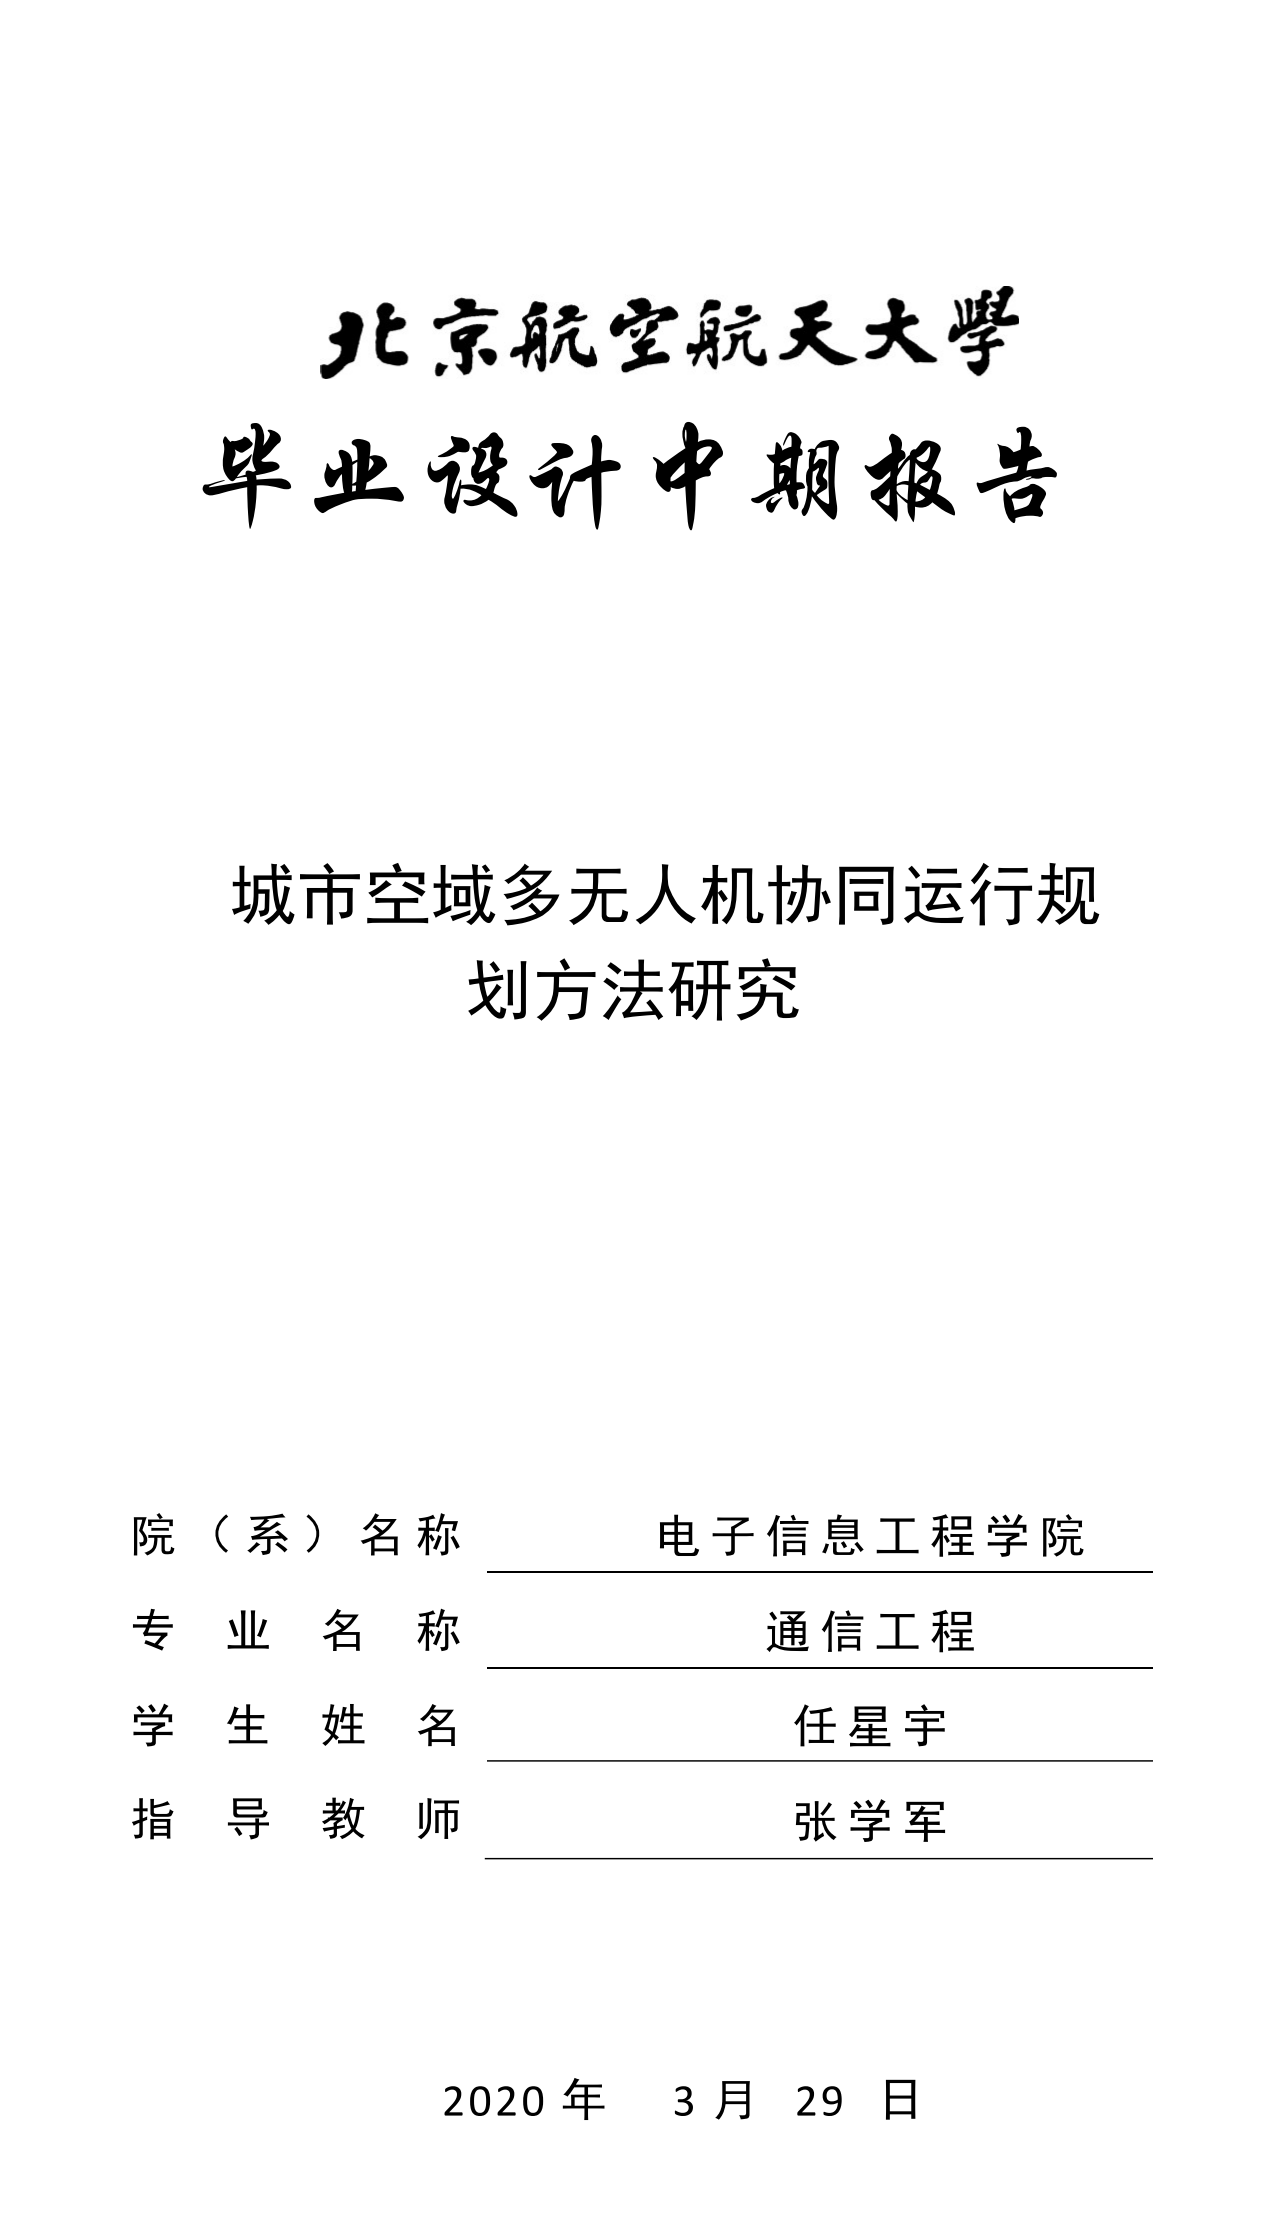
\includegraphics{titlepage.png}
\end{figure}
\thispagestyle{empty}
\newpage


\tableofcontents
\thispagestyle{empty}
\newpage

\begin{figure}[ht]
    \centering
    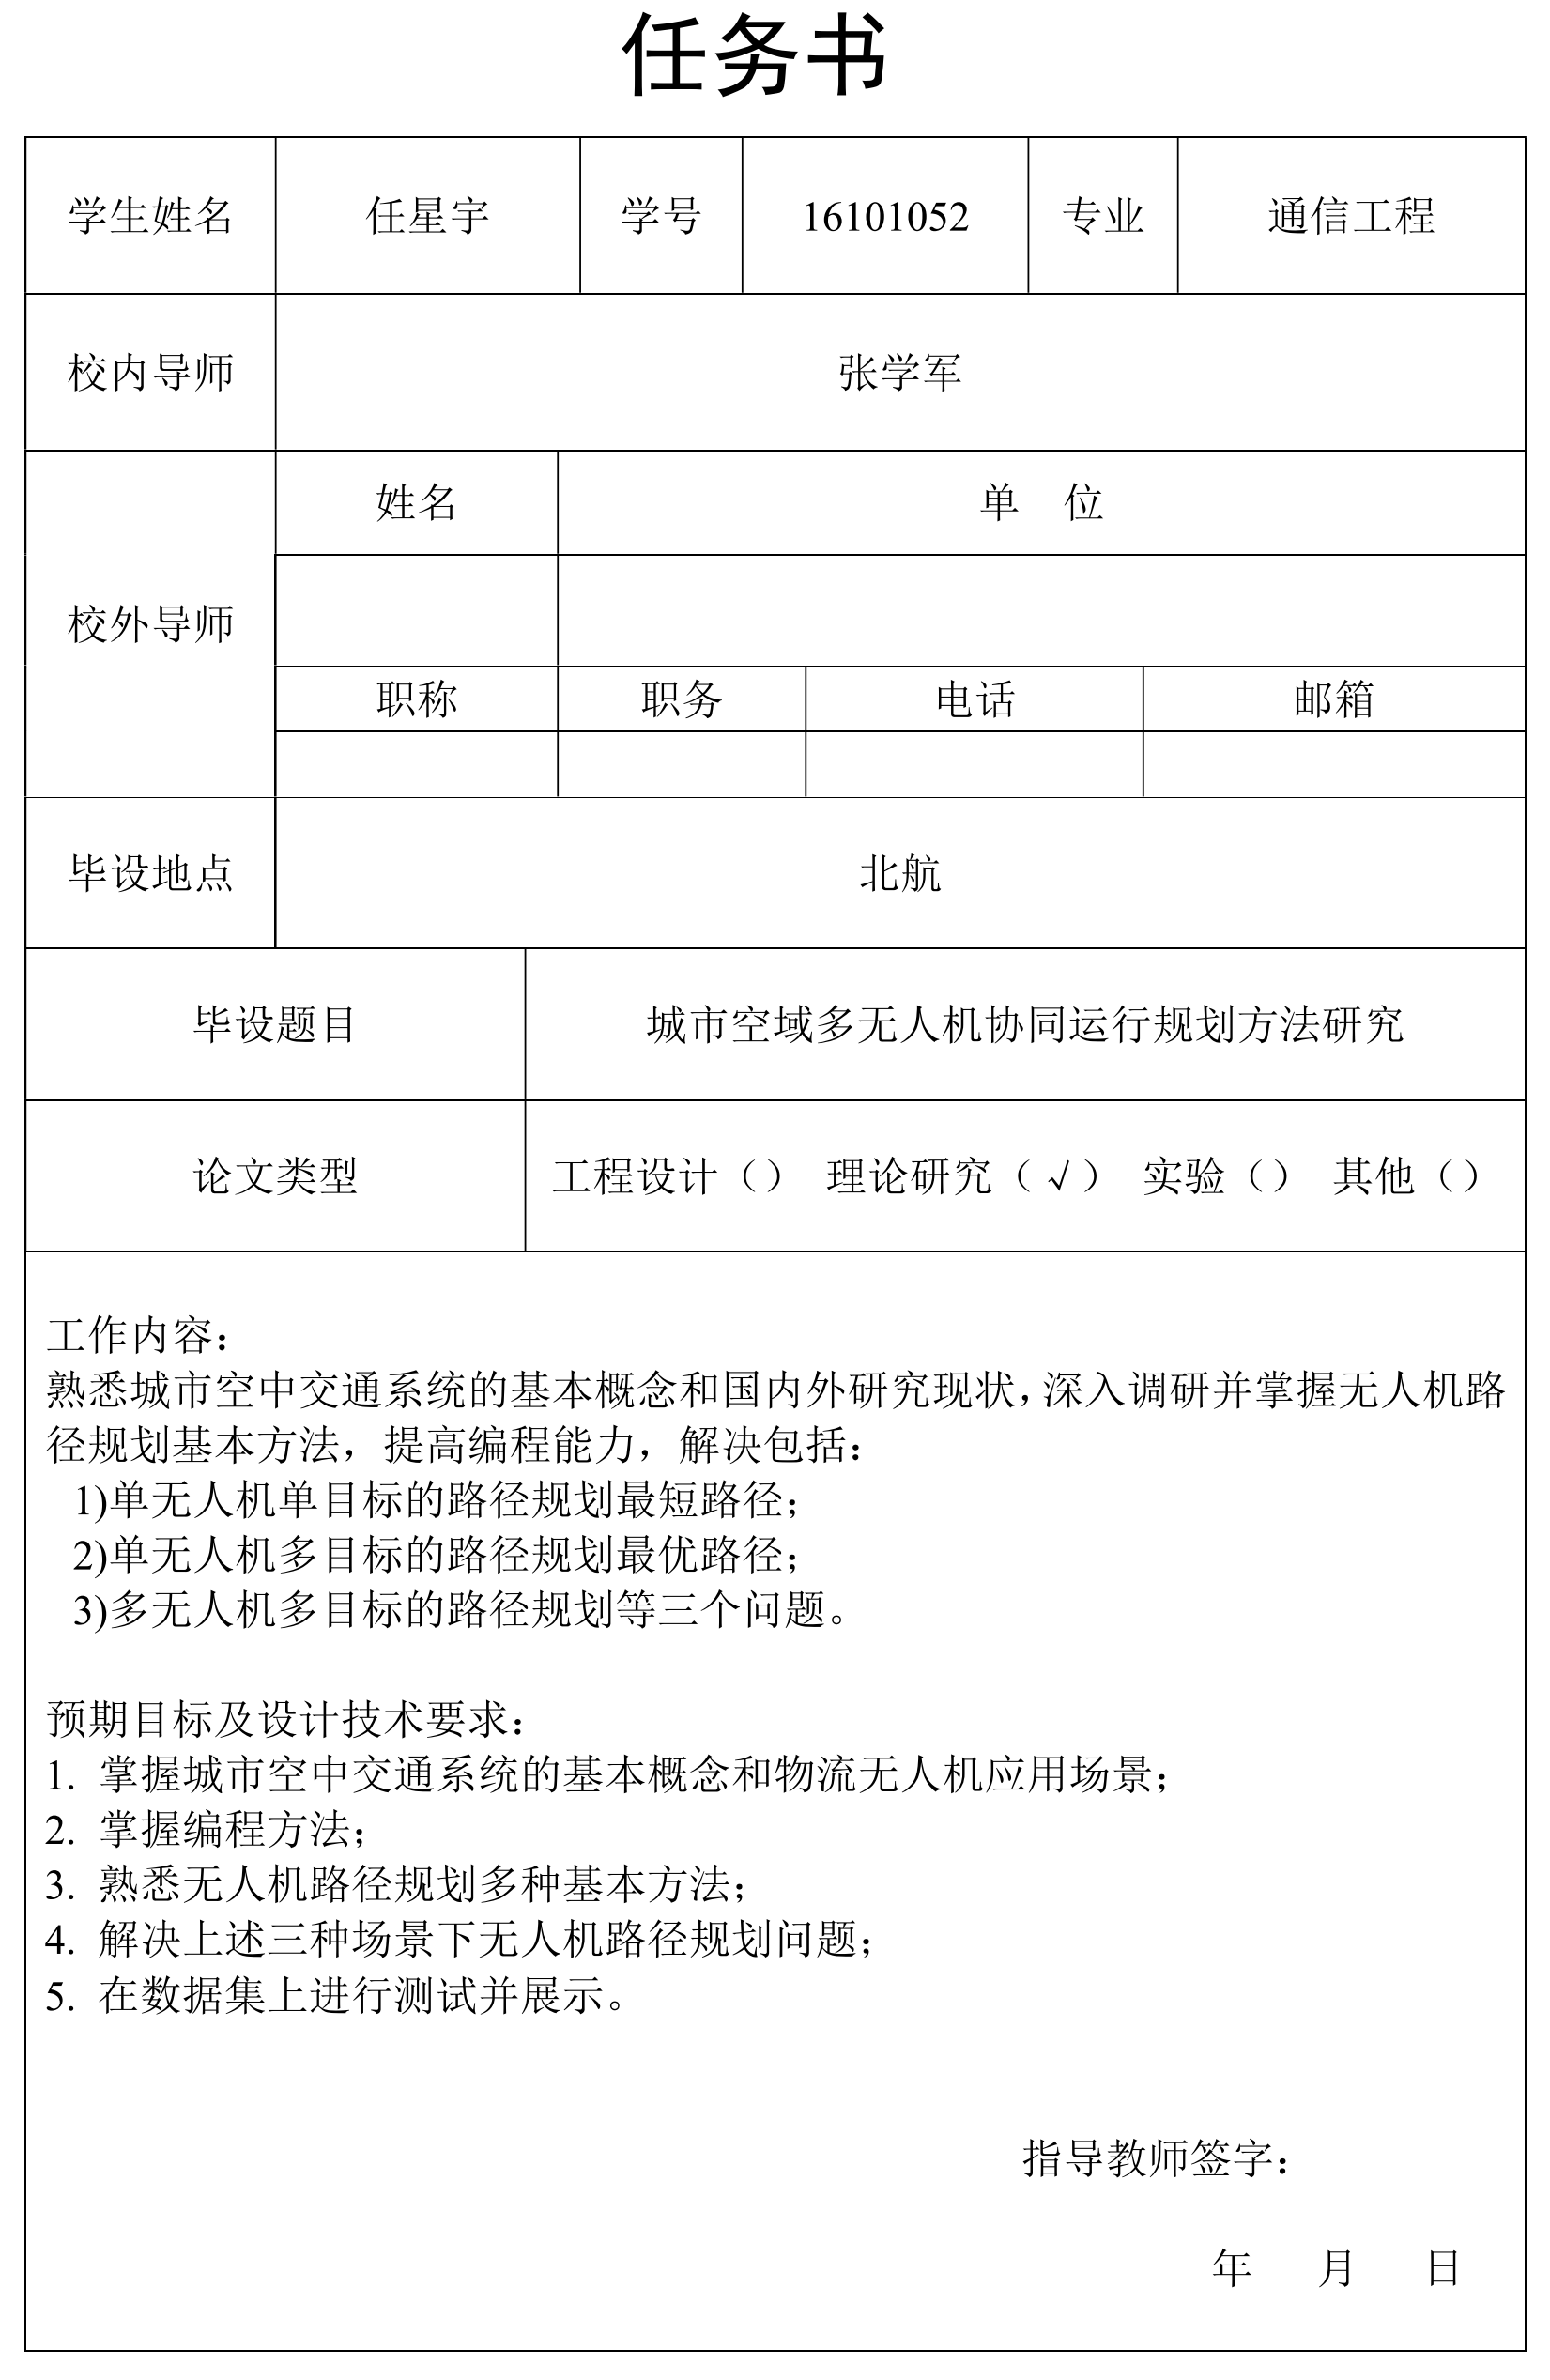
\includegraphics[scale=0.75]{renwushu.png}
\end{figure}
\thispagestyle{empty}
\newpage

\pagestyle{fancy}		%使用fancy页面风格
\rhead{}
\chead{北京航空航天大学电子信息工程学院}			%设置页眉中间
\lhead{}
% \lfoot{\rightmark}			%设置页脚左侧为rightmark
\cfoot{\thepage}			%设置页脚中间为页码
\newpage
\section{毕设工作简介}
\setcounter{page}{1}
\subsection{课题来源、研究目的及意义}
\paragraph{}近年来低空无人机发展迅速,根据中国民航局2019年第一季度无人机云数据统计:运行高度在120m以下的无人机占96.5\%,1000m以下的无人机占据99.9\%.无人机从某特定地点起飞,按照任务要求在复杂空域内运行并到达指定目的地,运行过程中不能给地面人类、空中交通参与者带来威胁,同时规避空域内障碍物风险、潜在威胁区域以及可能的飞行冲突问题,最终满足无人机飞行代价最低~\cite{kopardekar2016unmanned}。
\paragraph{}要解决上述问题,首先,要开展无人机运行安全风险评估研究,从地面、空中两个角度衡量无人机运行所带来的安全隐患,在满足安全性前提下获取无人机自身目标安全水平,评估运行空域的安全状态并生成空域危险等级;其次,基于无人机自身目标安全水平以及空域安全态势要求,开展单架无人机自主飞行路径规划研究,针对二维、三维不同运行场景参数限制,有效规避地形障碍物、空域潜在威胁等因素,为无人机规划最优运行路径;第三,在解决单架无人机最优化运行的基础上,研究多无人机协同路径规划问题并考虑时间因素,在实现无人机自身影响因素建模的前提下,重点解决多无人机时空协同运行问题、飞行冲突及间隔保持问题,为每架无人机规划时空最优运行路径。针对单架无人机路径规划场景数据量大、作用因素多且关联性强、全局范围内寻优复杂等诸多难点问题,首先,根据无人机运行任务需求设计一种离散化的路径特征提取机制,将此类问题转化为多目标大尺度下的联合全局优化,然后构造地形函数并完成所有影响因素的建模;其次,将无人机飞行距离、飞行时间等均作为约束条件,设计目标优化函数并在搜索空间内为其分配搜索阈值;第三,基于指定地形特征及影响因素作用开展最优化运行研究,提出两类适用于二维/三维不同场景下的高效路径规划算法,实现最优解位置的快速定位并得到最优运行路径点序列,实验结果证明算法具有较好的有效性、精确性与鲁棒性。针对多无人机运行规划中自身限制因素建模难、四维协同运行规划难等突出问题~\cite{liuyang}。
\paragraph{}例如亚马逊等公司开发的无人机物流配送即为其中一种应用场景,本课题的背景也是基于物流配送的低空无人机,意图初步实现一种物流管理和路径规划方案。低空环境更接近于路面的路径,但是低空无人机可以经过的空间是三维的,相对地面的车辆,路径限制更少。
\subsection{国内外研究现状}
\paragraph{}关于路径规划,有经典的算法和近年来发展的算法。 经典的算法是基于图论的组合优化问题。涉及的经典算法包括 Dijkstra 算法,Floyd-Warshall 算法,流问题的 Ford-Fulkerson 方法~\cite{introtoalgo}。近年来在经典算法方向的研究也包括利用组合优化的方法,利用整数规划,动态规划等方法,进行路径的规划~\cite{introtoor}。这种方法的原理是在规划空间内用一系列的路径段表征一条运行路径,通过搜索算法寻找最优的路径段实现无人机最佳运行路径的获取,该方向已经成为研究的热点。通过使用 Voronoi 图实现了飞行器的运行规划,此方法是把危险区域、无人机均等同于一个质点并建立 Voronoi 图,然后通过 K 算法寻找最优路径,由于该算法并未涉及无人机自身的参数性能因素,并不符合实际的运行 要求,因此无法真正应用到实际场景中;又进一步的将该算法扩展到了无人直升机的运行规划领域,而且收到了较好的效果,PRM 算法的核心是通过在运动的空间内实施采样,通过采样结果生成路线图,然后基于该路线图进行路径的进一步搜索后得到最佳路径,主要分为学习阶段、查询阶段两个过程;还有一种方法叫可视图法(Visibility Graph, VG)~\cite{2005coordination},将障碍物、危险区域的顶点作为可视图基本元素,由互相可见的顶点生成路线 图,该方法原理简单,执行起来并不复杂,但是当区域内的危险区域、障碍物较多时, 算法的效率急剧下降,需要耗费大量的计算时间;Canny 早在 1987 年就提出了一种 叫做轮廓图的路线图理论,通过映射将高维度规划空间转化为低维度,在低维空间内 找出障碍物对应的边界,即轮廓,然后反复迭代最终得到一维轮廓曲线,进而获取最终的运行路径,该方法的缺陷是当问题维数较高时需要进行多次映射,导致运算量大、耗时长,此方法并不是十分实用;还有一种概率地图法~\cite{zhangyi2007j},在无人机自主运行规划中得 到了广泛的应用,通过该方法使得规划问题的复杂度与规划空间的复杂度不受规划空间维数的影响,因此即使规划空间维度很高时也不会影响算法的执行效率,运算时间几乎不受影响 基于组合优化的经典算法研究在于精确(或较精确)的求解问题,可以保证最优(或对于 NP 难问题求近似最优)~\cite{chenyan2009}。
\paragraph{}而另一种思路和方向是通过类似统计和估计的近似算法,包括蚁群算法,PSO 算法,以及启发式的算法,例如A*算法。这些算法的特点是结果未必正确,精确性和模型个体相关性较大,与计算参数和计算机效果相关性很大,甚至从其算法目的上来说,其追求的就是“近似最优”。 近些年的另一种研究思路是通过人工智能的方法研究路径规划。

\subsection{研究内容简介}
\subsubsection{问题的简述}
\paragraph{}对于地面路径规划的研究已有不少,所以对于无人机的路径规划,其实有其一般性,但是由于无人机这一特殊的对象以及其所运行的环境的不同,这一问题又有其特殊性。
\paragraph{}无人机所运行的环境与地面的路径很多不同,包括\begin{itemize}
    \item 在一些空间内,障碍物并不多,所以我们完全可以用两点之间线段最短来解决这个问题;如果在此环境中使用较为密集的数据单元结构进行计算,那么计算量很大,而且肯定不会比直线段有更近的距离
    \item 在一些环境中,无人机并不是完全自由的,除了建筑物等障碍物之外,由于各种禁飞区和人员密集区的安全考虑,可自由飞行的区域要大打折扣。
\end{itemize}
\subsubsection{图的描述}
\paragraph{}有常见的几种图的表示方法,如下。
\begin{itemize}
    \item 栅格图\label{grid}
          \paragraph{}
          栅格图是一些由特定大小的立方体塞满整个空间的一种图的表示方法,一个立方体有6或8或更多的可运行方向,表示无人机可以从一个方格运行到另一个方格的方向。这种图的好处在于格子之间的路径是确定的,比如对于坐标轴方向的移动,耗费的距离为$a/2$,其中$a$是立方体的边长。但这种图的结构带来的很严重的问题就是数据密度过大,对于一个各个边有100个立方体组成的边来说,它的节点的数量级就已经超过了$10^6$,这种数量是难以进行计算的。但是,如果我们想要以更低的数据密度来进行计算,带来的问题是严重的,比如在一个过大的栅格中有很多房屋,对于无人机配送来说就有很大的误差~\cite{gridsgraph}。
    \item 无向图
          \paragraph{}给定一个图$G=(V,E)$,其中$V$表示的是图的顶点,对应于无人机在运行中需要经过的节点,$E$表示节点之间的边,这是一种最简单的图模型。这种图相对于栅格图,具有更高的抽象,更适合作为数学的研究对象。就其定义而言,顶点的名字在当前并不重要,我们需要的是一个之地啊这些顶点的方法,使用$0,...,V-1$来表述咯咯地那个点。这样描述是为了方便使用数组的索引进行节点的访问,我们知道,在计算机中,数组中下标为$i$的节点的访问速度是$O(1)$,关于这种表示相对于实际生活的差距问题,我们在后续的API中进行处理。无向图其实已经不错,对于大多数问题来说已经够了,图中的节点并不是栅格图中的相邻方格,而是表示某一个地理上的节点,比如一处房屋,或者一个物流配送点。这相对于栅格图有更小的数据密度而不至于失去精确性~\cite{introtoalgo}。
          \paragraph{}
          但是对于生活中的一些问题,无向图又有了缺点。比如车辆上坡和下坡的时间消耗和油耗是不同的,即使是同一条路。这就引出了有向图
    \item 有向图
          \paragraph{}有向图中地每一条边都是有方向的,不仅可以很好地描述各个抽象节点之间地距离,而且可以描述更多地问题,比如单行道,比如同一段上下坡路的不同代价。
          \paragraph{}关于有向图,也有很多研究的形式,我们在这里采用如下规定:
          \begin{itemize}
              \item 没有负边
              \item 不考虑自环
          \end{itemize}
\end{itemize}


\subsubsection{单无人机的单目标路径规划}
\paragraph{}这个问题的主要内容是考虑一个简单的配送站,在规定只有一个目标的情况下,如何从源节点(配送站)将货物送达目标的最优方案问题。
\paragraph{}关于最短路径的算法,有很多精确的经典算法,比如Dijkstra算法~\cite{felner2011position}和Bellman-Ford算法~\cite{bellman1958routing}。
\paragraph{Dijkstra算法}Dijkstra算法能够解决边权重非负的加权有向图的单起点最短路径问题。其运行的时间复杂度是$O(E\log{V})$.
\paragraph{Bellman-Ford算法}本算法能够解决包含负权重边的加权有向图的单起点最短路径问题。时间复杂度是$O(EV)$.
\paragraph{}对于我们的问题的模型是没有负权重边的,加上时间的考虑,最终使用了Dijkstra算法。其实现见~\ref{sec:dijkstra}.

\paragraph{A*算法}一种启发式的单节点最短路径的算法,关于种种解决方案并没有具体的时间复杂度,但是这种方案有很大的弊端,其一是基于栅格图~\ref{grid}的缺陷,数据密度过大,有很多冗余,使得算法运行非常慢;其二是算法是启发性的,往往并不能得到最短的路径,只是相对短的路径~\cite{astarredbloggames}。


\subsubsection{单无人机的多目标路径规划}
\paragraph{准备}在考虑正式的问题之前,我们先实现一些工具方法。
\subparagraph{Floyd-Warshall算法}Floyd-Warshall 算法采用动态规划方案来解决在一个有向图 $G = (V, E)$ 上每对顶点间的最短路径问题,即全源最短路径问题(All-Pairs Shortest Paths Problem),其中图 $G$ 允许存在权值为负的边,但不存在权值为负的回路。Floyd-Warshall 算法的运行时间为 $Θ(V^3)$。
\subparagraph{}Floyd-Warshall 算法由 Robert Floyd 于 1962 年提出,但其实质上与 Bernad Roy 于 1959 年和 Stephen Warshall 于 1962 年提出的算法相同。其实现见~\ref{sec:floydsolution}.


\paragraph{TSP问题}在存在多个目标的情况下,可以抽象为TSP问题~\cite{tsptheory},又称旅行商问题。给定一系列节点和每对节点之间的距离,求解访问每一座节点一次并回到起始节点的最短回路。它是组合优化中的一个NP困难问题,在运筹学和理论计算机科学中非常重要。已知TSP算法最坏情况下的时间复杂度随着节点数量的增多而成超多项式(可能是指数)级别增长。
\subparagraph{}问题在1930年首次被形式化,并且是在最优化中研究最深入的问题之一。许多优化方法都用它作为一个基准。尽管问题在计算上很困难,但已经有了大量的启发式和精确方法,因此可以完全求解节点数量上万的实例,并且甚至能在误差1\%范围内估计上百万个节点的问题。
\subparagraph{}甚至纯粹形式的TSP都有若干应用,如企划、物流、芯片制造。稍作修改,就是DNA测序等许多领域的一个子问题。在这些应用中,“节点”的概念用来表示客户、焊接点或DNA片段,而“距离”的概念表示旅行时间或成本或DNA片段之间的相似性度量。TSP还用在天文学中,观察很多源的天文学家希望减少在源之间转动望远镜的时间。许多应用(如资源或时间窗口有限)中,可能会加入额外的约束~\cite{worldtsp}。
\subparagraph{}TSP问题可以通过整数规划的方法解决~\cite{papadimi},目前还没有进行整数规划的学习,暂将方程列下:
\begin{align*}
    \min & \sum _{i=1}^{n}\sum _{j\neq i,j=1}^{n}c_{ij}x_{ij}\colon &  &                      \\
         & x_{ij}\in \{0,1\}                                        &  & i,j=1,\ldots ,n;     \\
         & u_{i}\in  \mathbb{Z}                                     &  & i=2,\ldots ,n;       \\
         & \sum _{i=1,i\neq j}^{n}x_{ij}=1                          &  & j=1,\ldots ,n;       \\
         & \sum _{j=1,j\neq i}^{n}x_{ij}=1                          &  & i=1,\ldots ,n;       \\
         & u_{i}-u_{j}+nx_{ij}\leq n-1                              &  & 2\leq i\neq j\leq n; \\
         & 0\leq u_{i}\leq n-1                                      &  & 2\leq i\leq n.
\end{align*}
\subparagraph{}关于TSP问题的是实现见~\ref{sec:solutionTSP}.
\subparagraph{应用场景}除了本文所述的物流规划问题,TSP问题在其他方面也有很多应用。比如飞机航线安排、送邮件、快递服务、设计校车行进路线等等。实际上其应用范围扩展到了许多其他领域。
\subparagraph{}印制电路板转孔是TSP应用的经典例子,在一块电路板上打成百上千个孔,转头在这些孔之间移动,相当于对所有的孔进行一次巡游。把这个问题转化为TSP,孔相当于节点.孔到孔之问的移动时间就是距离。
\subparagraph{}此外,旅行商问题还有电缆和光缆布线、晶体结构分析、数据串聚类等多种用途。更重要的是.它提供了一个研究组合优化问题的理想平台。很多组合优化问题,比如背包问题、分配问题、车间调度问题都和TSP同属NP完全问题,它们都是同等难度的.如果其中一个能用多项式确定性算法解决,那么其他所有的NP完全问题也能用多项式算法解决。很多方法本来是从TSP发展起来的.后来推广到其他NP完全问题上去~\cite{tsp2006}。

\subsubsection{多无人机的多目标路径规划}
\paragraph{}多无人机的路径规划涉及的主要问题是车辆路径规划问题(Vehicle Routing Problem),是TSP问题的一般化,相对来说更接近实际的模型,但是也复杂得多。鉴于TSP问题是一个NP难的问题,因此VRP问题也是一个NP难的问题。

\paragraph{VRP问题}最早是由Dantzig和Ramser于1959年首次提出~\cite{dantzig1959truck},它是指一定数量的客户,各自有不同数量的货物需求,配送中心向客户提供货物,由一个车队负责分送货物,组织适当的行车路线,目标是使得客户的需求得到满足,并能在一定的约束下,达到诸如路程最短、成本最小、耗费时间最少等目的。
基本问题的方程如下:
\begin{align*}
    \min & \sum_{i\in V}\sum_{j \in V}c_{ij}x_{ij}\colon   &  &                                                     \\
         & \sum _{i\in V}x_{ij}=1                          &  & \forall j\in V\backslash \left\{0\right\}           \\
         & \sum _{i\in V}x_{ij}=1                          &  & \forall j\in V\backslash \left\{0\right\}           \\
         & \sum _{i\in V}x_{i0}=K                          &  &                                                     \\
         & \sum _{j\in V}x_{0j}=K                          &  &                                                     \\
         & \sum _{i\notin S}\sum _{j\in S}x_{ij}\geq r(S), &  & \forall S\subseteq V\setminus \{0\},S\neq \emptyset \\
         & x_{ij}\in \{0,1\}                               &  & \forall i,j\in V
\end{align*}
\subparagraph{变种问题}可见,VRP问题考虑的实际状况要复杂得多,VRP问题涉及的变种问题也有很多~\cite{vrpweb},包括:
\begin{itemize}
    \item VRP 基本的VRP问题,不涉及更多的条件。这往往和实际情况相差太多。
    \item Capacitated VRP (CPRV) 设每辆车有容量限制,在容量限制内运输货物
    \item VRP with Profits (VRPP) 车辆的运输有运出成本和收益
    \item VRP with Pick-Up and Delivering (VRPPD) 不是单货源的情况,多个取件(Pick-Up)点和多个收件(Delivering)点
    \item VRP with Time Window (VRPTW) 每个客户的收货时间是有限的,须在某个时间段内配送。
\end{itemize}
\subparagraph{模型选择}无人机的配送目前并不是应用在大宗商品的远距离运输上,更聚焦于单个配送站对多个点进行短距离配送。在短途配送的过程中,配送客户的收货时间往往是较为固定的,并不是大宗商品运输中的严格时限,大多数快递等货物的订单签收往往发生在中午后者晚上,在周末往往有更宽的时限。无人机的电量和补给相对来说也很重要,但是鉴于复杂性,本文最终采用CVRP问题。

\subparagraph{}VRP问题有很多解法,在关于VRP问题的进一步描述和探究见~\ref{sec:vrp}

\paragraph{综述} 综合来说,实际问题可定义为这样一个模型:从中心配送站$O$像多个配送点配送快递,快递的重量不同,无人机的载重是一定的。在每天的某个固定时间段,向大量客户位置进行配送,需使用VRP问题的模型解决问题,对于少数特殊客户,在该时间段内无法收货,则单独对其在另一时间段进行配送。






\section{预处理和工具}
我们首先需要预处理一些数据,将现实生活中的问题抽象为可计算的模型。
\subsection{图的抽象}
如何描述一个实际地图中的配送点位置和之间的关系,是建模的首要问题。在普遍的数学模型中,我们应考虑使用有向图进行建模。这种好处在于:有向图可以完整描述点之间的关系,包括一些特殊情况下两点之间的来回不等的情况(实际上这种情况往往是常见的,可能有些路径是单向路径,有些路径类似于上下坡,来回的成本自然不同)。
\subsubsection{有向图}
\subparagraph{}进一步地描述一下有向图。有向图的接口包括的方法如表~\ref{tab:edgewg}所示。
\begin{table}[htbp]
    \centering
    \caption{加权有向图}\label{tab:edgewg}

    \begin{tabular}{R{1.5cm}L{8cm}L{5cm}}
        \hline
        \hline
        interface & \textbf{EdgeWeightedDiGraph}                                                                   \\
                  & \multicolumn{2}{l}{implements \textbf{SymbolGraphAPI}, \textbf{RealMapGraph}}                  \\
        \hline
                  & V()                                                                           & 顶点数         \\
                  & E()                                                                           & 边数           \\
                  & addEdge(\textbf{WeightedDirectedEdge} edge)                                   & 添加边         \\
                  & adjOf(int v)                                                                  & 顶点所连接的边 \\
                  & reverse()                                                                     & 图的反向图     \\
        \hline
    \end{tabular}
\end{table}

\subsubsection{有向边}其中的\textbf{WeightedDirectedEdge}是有向边的接口,其实现了的方法如表~\ref{tab:weightedDiEdge}所示。
\begin{table}[htbp]
    \centering
    \caption{加权有向边}\label{tab:weightedDiEdge}

    \begin{tabular}{R{1.5cm}p{8cm}p{5cm}}
        \hline
        \hline
        interface & \textbf{WeightedDirectedEdge}                \\
        \hline
                  & from()                        & 边指出的节点 \\
                  & to()                          & 边指向的节点 \\
                  & weight()                      & 边的权重     \\
        \hline
    \end{tabular}

\end{table}
\subparagraph{}关于接口\textbf{SymbolGraphAPI}, \textbf{RealMapGraph}的描述见~\ref{sec:graphAPI}所述



\subsection{抽象图的具体化\label{sec:graphAPI}}
\subsubsection{符号图}生活中的图都是以名称(某一个字符串)作为节点的表示的,对于上述使用整数表示的节点,显然是不合实际的,所以引入了关于符号图的接口,其表述了图和某个地名(字符串类型)的一一映射的关系。实现建议使用哈希表进行快速插入和查询。其接口见表~\ref{tab:symbolGraph}.
\begin{table}[htbp]
    \centering
    \caption{符号图}\label{tab:symbolGraph}
    \begin{tabular}{R{1.5cm}p{8cm}p{5cm}}
        \hline
        \hline
        interface & \textbf{SymbolGraphAPI}                                                \\
        \hline
                  & indexOf(String vertex)           & 获得和某个节点名字 相关联的节点索引 \\
                  & nameOf(int v)                    & 得到和某个索引相关 联的名字         \\
                  & setIndexOf(String vertex, int v) & 设置节点                            \\
        \hline
    \end{tabular}
\end{table}
\subsubsection{坐标}关于类似A*算法或者某些启发式算法等图的算法需要进行对于坐标的描述。所以引入了关于坐标的接口,如表~\ref{tab:coordination}所示。
\begin{table}[htbp]
    \centering
    \caption{坐标}\label{tab:coordination}
    \begin{tabular}{R{1.5cm}p{8cm}p{5cm}}
        \hline
        \hline
        interface & \textbf{Coordination}                                                           \\
        \hline
                  & dist(\textbf{Coordination} that)          & 当前节点到另一个\textit{that}的距离 \\
                  & setX(int x),getX(),etc.                   & 直角坐标的获取和设置                \\
                  & getR(),getPhi()                           & 获得极坐标                          \\
                  & relativeCoordinationOf(Coordination that) & 相对坐标                            \\
        \hline
    \end{tabular}
\end{table}


\subsection{图的表示}
\subsubsection{邻接矩阵}
\paragraph{}我们通常会将图 G中的结点编为$1,2,...,|V|$,这种编号可以是任意的。在进行此种编号之后,图 $G$的邻接矩阵表示由一个 $|V|\times|V|$的矩阵$A=(a_{ij})$予以表示,该矩阵满足下述条件:
\[
    a_{ij}=\begin{cases}
        w(i,j) & if(i,j)\in E \\
        \infty & others
    \end{cases}
\]
无向图的邻接矩阵是一个对称矩阵。由于在无向图中,边$(u,v)$ 和
边$(v, u)$是同一条边,无向图的邻接矩阵$A$就是自己的转置,即$ A=A^T$。在某些应用中,可能 只需要存放对角线及其以上的这部分邻接矩阵(即半个矩阵),从而将图存储空间需求减少几乎 一半。
与邻接链表表示法一样,邻接矩阵也可以用来表示权重图。例如,如果 $G = (V,E)$为一个 权重图,其权重函数为切,则我们直接将边$(u, v)\in E$ 的权重 $w(u,v)$ 存放在邻接矩阵中的第 $u$ 行第$v$ 列记录上。对于不存在的边,则在相应的行列记录上存放值 NIL. 不过,对于许多问题来 说,用 0 或者$\infty$来表示一条不存在的边可能更为便捷。
虽然邻接链表表示法和邻接矩阵表示法在渐近意义下至少是一样空间有效的,但邻接矩阵 表示法更为简单,因此在图规模比较小时,我们可能更倾向于使用邻接矩阵表示法。而且,对于 无向图来说,邻接矩阵还有一个优势:每个记录项只需要 1 位的空间。
\subsubsection{邻接链表}
\paragraph{}对于图$G=(V,E)$来说,其邻接链表表示由一个包含$|V|$条链表的数组$adj$所构成,每个节点有一条链表。对于每个节点$u\in V$,邻接链表$adj[u]$包含所有与节点$u$之间有边相连的含有有向权重边。有向图中邻接链表表示法的存储空间需求平均为$O(V+E)$.邻接链表表示法的鲁棒性很高,可以对其进行简单修改来支持许多其他的图变种。
\paragraph{}邻接链表的一个潜在缺陷是无法快速判断一条边$(u, v)$是否是图中的一条边,唯一的办法是在邻接链表$adj[u]$里面搜索结点。相比邻接矩阵就差得多了。

\subsection{拓展数据结构}
\subsubsection{带索引的优先队列~\cite{algs4}}\label{sec:indexedpq}
\paragraph{}优先队列表示了一组值和对这些值的操作,能够以较快速度得到最值和对最值操作。
\paragraph{}经常使用的优先队列支持的操作一般是:插入,返回最小,删除最小。Java自带的优先队列就是这样的。但是在图论中使用的优先队列要求有对某个元素更新的操作,如果使用普通的优先队列, 难以实现在对数时间内进行更改的操作,所以我们进行了修改,使用带索引的优先队列,给每个队列中的元素以某个索引(是图中的节点编号)链接,这样在修改时,只需进行相应位置的元素更改(数组元素更改),并进行上浮和下沉操作。
\paragraph{}其伪代码见算法~\ref{algoindexedpq}

\subsection{基本图论工具}
\subsubsection{强连通分量}\label{sec:scc}
\paragraph{}许多针对有向图的算法都以此种分解操作开始。在将图分解为强连通分量后,这些算法将分别运行在每个连通分量上,然后根据连通分量之间的连接 结构将各个结果组合起来,从而获得最终所需的结果。
\paragraph{定义}强连通元件(英语:Strongly connected component)是图论中的概念。图论中,强连通图指每一个顶点皆可以经由该图上的边抵达其他的每一个点的有向图。意即对于此图上每一个点对$(u,v)$,皆存在路径$u\to v$以及$v\to u$.
\paragraph{}我们用于寻找强连通分量的算法需要用到图 $G=(V, E)$的转置,将其定义为 $G^T=(V,E^T)$,这里 $E^T=\{(u, v): (v, u) \in E\}$。也就是说, $E^T$ 由对图 $G$中的边进行反向而 获得。给定图 $G$的邻接链表,创建 $G^T$的时间为 $O(V+E)$.
\paragraph{}其伪代码见算法~\ref{scc}.


\section{单无人机的单目标规划}
对于较特殊的配送客户,配送往往不在时间段内,所以只能单独配送,对于单独配送,我们使用Dijkstra算法。
\subsection{Dijkstra算法}\label{sec:dijkstra}
\paragraph{算法描述}Dijkstra算法解决的是带权重的有向图上单掠最短路径问题,该算法要求所有边的权重都为 非负值。因此,在本节的讨论中,我们假定对于所有的边$(u,v)\in E$,都有 $w(u,v)\geq 0$。我们稍后将看到,如果所采用的实现方式合适, Dijkstra 算法的运行时间要低于 Bellman-Ford 算法的运行时间。
\subparagraph{}Dijkstra算法在运行过程中维持的关键信息是一组结点集合 {$S$}. 从源结点 {$s$} 到该集合中每个 结点之间的最短路径已经被找到。算法重复从结点集 $V-S$ 中选择最短路径估计最小的结点 $u$, 将 $u$加入到集合$S$,然后对所有从 $u$ 发出的边进行松弛。在下面给出的实现方式中,我们使用一个最小优先队列 $Q$来保存结点集合,每个结点的关键值为其$d$值。
\subparagraph{使用的数据结构}在这里使用的优先队列是一个带索引的优先队列,索引的好处在于很好地和图地节点(整数)进行结合,更多优势见~\ref{sec:indexedpq}。另一种很好地方式是使用普通的优先队列,但需要一个节点类,其需要包含节点和距离两个信息,并以距离作为Comparable接口的参数。
\paragraph{伪代码}见~\ref{algodijkstra}

\section{单无人机的多目标规划}
\subsection{TSP问题的拓展}\label{sec:tspEXT}
\paragraph{}TSP问题中要求我们经过每个节一次,但是实际问题中,更适合的是“至少一次”。很多情况下,允许多次经过一个节点会得到更短的路线。
\paragraph{}考虑三个点$u,v,w$的路径矩阵如下:
\[
    A=\begin{pmatrix}
        0 & 1  & 2  \\
        1 & 0  & 10 \\
        2 & 10 & 0
    \end{pmatrix}
\]
\paragraph{}如果初始从$u$节点出发,出发往$v$,在前往$w$时,如果不允许经过节点$u$时,其路程为10,如果允许经过节点$u$,那么就是3。所以最终将问题的模型为至少访问一次。

\subsection{Floy-Warshall算法}\label{sec:floydsolution}
\paragraph{算法描述}如前所述,Floyd算法是一种基于动态规划思想的算法。
\subparagraph{}对于任意节点对$i,j\in V$,考虑从节点$i$到节点$j$的所有中间节点全取自于集合$\{1,2,...,k\}$的路径,并且设$p$为齐总权重最小的路径。算法利用了路径$p$和从$i$到$j$之间中间节点均取自于集合$\{1,2,...,k-1\}$的最短路径之间的关系。这种关系依赖于节点$k$是否是路径$p$上的一个中间节点。
\begin{itemize}
    \item 如果是,则路径$p$上所有中间节点都属于集合$\{1,...,k\}$,则对于前后两个节点集合的结果是相同的。
    \item 如果不是,将路径分解为两部分:从$i$到$k$和从$k$到$j$的最短路径。
\end{itemize}
\paragraph{递归解}设$d_{ij}^{(k)}$是从节点$i$到节点$j$的所有中间节点全部取自于集合$\{1,2,...,k\}$的最短路径的权重。得到下面的递归解:
\[
    d_{ij}^{(k)}=\begin{cases}
        w_{ij}                                             & if~ k=0     \\
        \min(d_{ij}^{(k-1)},d_{ik}^{(k-1)}+d_{kj}^{(k-1)}) & if~ k\geq 1
    \end{cases}
\]
\subparagraph{}可以使用自底向上的动态规划的方法将上述递归求解的思路转化为迭代求解,其时间复杂度减少至$O(V^3)$.
\subparagraph{}关于构建路径树的方法,可以使用一个数组同时在计算最短路径的时候,实现记录前驱的方法。其中,前驱的递归表示如下:
\[
    \Pi_{ij}^{(k)}=\begin{cases}
        \Pi_{ij}^{(k-1)} & if~ d_{ik}^{(k-1)}+d_{kj}^{(k-1)} \geq d_{ij}^{(k-1)} \\
        \Pi_{ik}^{(k-1)} & others
    \end{cases}
\]
\subparagraph{}其表示的是,对于从$i$到$j$的路径中,在前$k$个节点中,如果包括第$k$个节点,那么就记录下从$i$到$j$需经过的第一个节点是$k$.
\paragraph{伪代码}见~\ref{algofloyd}
\paragraph{遍历集合}设置一个参数为需遍历的集合,该集合未必是所有图中的节点,可以只是一部分(往往也是如此),这样可以使用上述Floyd-Warshall算法事先计算出一个邻接矩阵,用来表示一个包括所有需遍历集合的子图。

\subsection{TSP的解法及测试}\label{sec:solutionTSP}
\subsubsection{TSP的精确算法}
\paragraph{测试数据集}下述的TSP问题的数据集来自于TSPLIB.~\cite{tsplib}~\cite{reinelt1991tsplib}
\subparagraph{}本文使用的几个数据和数据的历史最佳数据,如表~\ref{tab:tsplib}
\begin{table}[htbp]
    \centering
    \caption[tspdata]{TSP数据集和最佳数据}\label{tab:tsplib}
    \begin{tabular}{R{5cm}L{5cm}}
        \toprule
        数据名  & 历史最佳 \\
        \hline
        ch130   & 6110     \\
        kroB200 & 29437    \\
        rat783  & 8806     \\
        pcb1173 & 56892    \\
        \bottomrule
    \end{tabular}
\end{table}
\paragraph{基本思路}TSP的精确解法有很多中,其中整数规划的方法暂时没有考虑,这里考虑的是一种递归的求解方法。考虑一个集合$S$,其表示的是所有需要经过的节点集合,点$u$设置为当前访问的节点。一旦我们访问过了节点$u$,就在下一次访问的时候去除掉该节点,即下次需要遍历的集合是$S-\{u\}$,这样对于需遍历的集合规模为$n$的集合来说,第一次选定了某个节点$i$之后,下次需访问的节点集合个数就变为了$n-1$,以此类推,我们得到所需访问的次数为$n!$.其递归的表示形式如下所示:
\[
    f(u,S)=\min(f(v,S-{u})|v\in adj[u])
\]

\subparagraph{}实际实践中,阶乘的时间复杂度是非常慢的,其实验结果如表~\ref{tab:tsprecurres}所示.
\begin{table}[htbp]
    \centering
    \caption{TSP递归的精确算法}\label{tab:tsprecurres}
    \begin{tabular}{R{7cm}L{7cm}}
        \toprule
        节点数 & 耗时   \\
        \hline
        10节点 & 1毫秒  \\
        11节点 & 1秒    \\
        12节点 & 14秒   \\
        13节点 & 1分钟  \\
        14节点 & 12分钟 \\
        \bottomrule
    \end{tabular}
    \begin{tablenotes}
        \footnotesize
        \item 测试电脑配置:1核CPU,2GB内存,CentOS 7.6 64位
        \item 测试数据集:随机生成
    \end{tablenotes}
\end{table}
\subparagraph{动态规划法}观察上述的递归方程式,胡发现其中很多计算具有冗余,我们可以考虑使用带记录的由上至下的递归方法解决这个问题,思路是通过一个名为$memo$的数组,记录当前节点$u$和当前待遍历集合$S$,初始化为$-1$,如果计算过了相关的节点,那么就直接返回该值,否则才进行计算。
\subparagraph{}其算法的复杂度为$O(n^22^n)$,其中$n$为待遍历集合的大小。

\subparagraph{引进工具类}正如前述~\ref{sec:tspEXT},TSP问题实际上有一个很严重的问题,即每个节点只能访问一次,这样就意味着可能走更远的距离。另一个问题是,在现实生活中的图会有很多节点,比如有1000个固定的配送点,但是我们在某次配送活动中需要配送的节点并不可能是全部,或许只有20个,所以我们在传入整个图作为计算参数的同时,还要传入一个节点集合$set$表示需要经过的点集。
\subparagraph{}因此我们考虑使用前述的Floyd-Warshall算法~\ref{sec:floydsolution},在原来图$G$的基础上构建一个二维矩阵$g$,其中的每一条边$(u,v)$都是由Floyd-Warshall算法算得的从$u$到$v$的最短路径$Dist(u,v)$. 这样就可以将前述两个问题一并解决。
\subparagraph{}另外我们可能需要考虑的问题是,给出的图$G$未必是强连通的图,而给出的遍历集合$set$中也未必是强连通的。所以我们可以考虑使用前述的强连通分量的算法~\ref{sec:scc},先确定$set$是否是强连通分量,否则不进行计算。

\paragraph{伪代码}见算法~\ref{algotspdp}~\cite{held1962dynamic}

\paragraph{测试结果}支持23点以下的计算量,过多的节点会导致空间消耗殆尽。结果如表~\ref{tab:tspdp}.
\begin{table}[htb]
    \centering
    \caption{TSP的精确算法:动态规划}\label{tab:tspdp}
    \begin{tabular}{R{7cm}L{7cm}}
        \toprule
        节点数 & 耗时          \\
        \hline
        19节点 & 90毫秒        \\
        20节点 & 800毫秒       \\
        21节点 & 2秒           \\
        22节点 & 12秒          \\
        23节点 & 21秒          \\
        24节点 & Out of Memory \\
        \bottomrule
    \end{tabular}
    \begin{tablenotes}
        \footnotesize
        \item 测试电脑配置:1核CPU,2GB内存,CentOS 7.6 64位
        \item 测试数据集:随机生成
    \end{tablenotes}
\end{table}

\subsubsection{TSP的贪心启发}
\paragraph{}在前述的精确解法中,其优势在于结果的准确性,但是由于指数级别的复杂度,无法计算较多节点,这是不现实的。我们可以考虑一种启发式算法。
\paragraph{}启发式算法常能发现很不错的解,但也没办法证明它不会得到较坏的解;它通常可在合理时间解出答案,但也没办法知道它是否每次都可以这样的速度求解~\cite{dantzig1954solution}。
\paragraph{} 有时候人们会发现在某些特殊情况下,启发式算法会得到很坏的答案或效率极差,然而造成那些特殊情况的数据组合,也许永远不会在现实世界出现。因此现实世界中启发式算法常用来解决问题。启发式算法处理许多实际问题时通常可以在合理时间内得到不错的答案。 有一类的通用启发式策略称为元启发式算法(metaheuristic),通常使用乱数搜寻技巧。他们可以应用在非常广泛的问题上,但不能保证效率。
\paragraph{}尽管启发式算法的结果往往具有随机性,其结果无法保障,但是只要不是特殊设计的数据集,其结果往往是比较靠谱的。
\paragraph{}首先使用一种最基础的启发式策略:贪心策略,这种启发式的方法和A*算法~\cite{astarredbloggames}的想法类似,维持一个未遍历的集合,在当前节点上,从未遍历集合中选择离当前节点最近的节点,访问该节点并置该节点为已访问,直到所有的节点都访问过。贪心启发的算法思路基于深度优先搜索。
\paragraph{伪代码}见算法~\ref{algogreedy}



\paragraph{测试结果}见表~\ref{tab:tspgreedy}
\begin{table}[htb]
    \centering
    \caption{TSP贪心启发}\label{tab:tspgreedy}
    \begin{tabular}{L{2cm}L{2cm}L{2cm}L{3.4cm}L{3.4cm}}
        \toprule
        数据名   & 节点数   & 耗时    & 结果  & 历史最佳          \\
        \hline
        随机生成 & 10节点   & 0毫秒   & 67    & 59.7 (准确结果) \\
        随机生成 & 20节点   & 0毫秒   & 164   & 81.2 (准确结果) \\
        ch130    & 130节点  & 10毫秒  & 7198  & 6110              \\
        kroB200  & 200节点  & 11毫秒  & 35394 & 29437             \\
        rat783   & 783节点  & 79毫秒  & 12008 & 8806              \\
        pcb1173  & 1173节点 & 240毫秒 & 69692 & 56892             \\
        \bottomrule
    \end{tabular}
    \begin{tablenotes}
        \footnotesize
        \item 测试电脑配置:1核CPU,2GB内存,CentOS 7.6 64位
        \item 测试数据集:TSPLIB
    \end{tablenotes}
\end{table}
\paragraph{}可见贪心启发确实速度极快,但是在很多测试结果上效果很不好。这是理论上合理的结果。在每次追逐最近结点的选择中,往往就会离另一些节点越来越远,长此以往,等到再次寻求这一节点的时候,就距离太远了。

\subsubsection{TSP的退火启发}
\paragraph{}贪心启发的方式非常简单直接,其结果往往也和准确结果相差甚远,因此引入一种改进的随机算法——模拟退火。模拟退火算法是一种随机化的贪心启发,在贪心搜索的过程中,做出的选择具有特定的随机性。模拟退火算法以一定的概率来接受一个比当前解要差的解,因此有可能会跳出这个局部的最优解,达到全局的最优解。
\paragraph{}其核心思想是:首先随机选择一个节点序列(在这里我选择了贪心的结果作为初始序列,以保证不会比贪心更差的结果,事实上,在后期的大量节点的图中,基本的退火算法并不比贪心的结果好多少),作为开始,接下来产生一个随机扰动,如果找到比上一个解更接近最优解的解,那么就直接接受这个解。而如果找到的解离得更远了,也以一定的概率接受。这个概率是根据Metropolis准则确定的,该准则的表述是
\[
    \exp\left(-\frac{\Delta}{t}\right)
\]
\paragraph{}该函数的性质如图~\ref{fig:metropolis}
\begin{figure}[htbp]
    \centering
    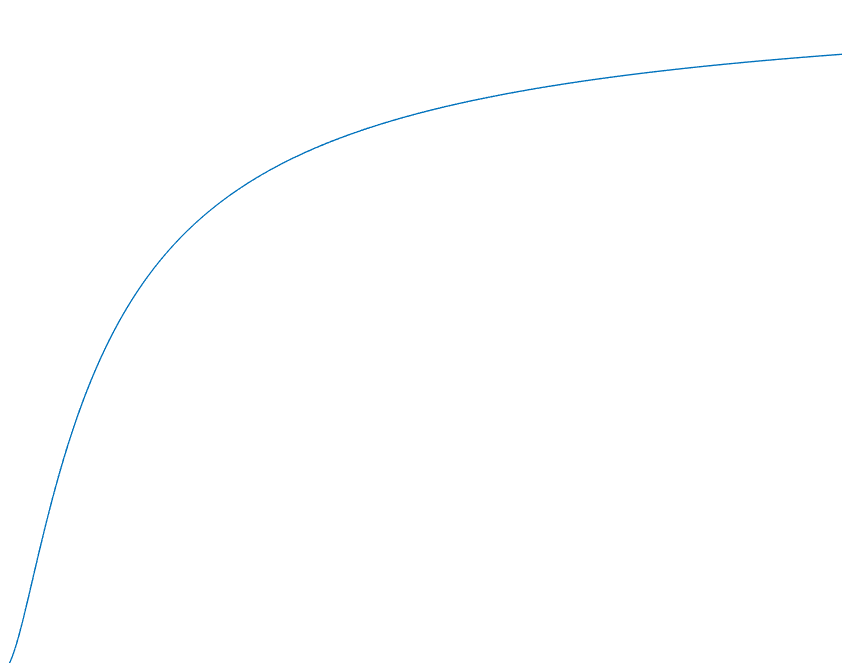
\includegraphics[scale=0.8]{metropolis.png}
    \caption{Metropolis准则}
    \label{fig:metropolis}
\end{figure}

\paragraph{}启发式算法的方式有很多种~\cite{arora1998polynomial},除了退火算法之外还有遗传算法,这些启发式的算法都是随机化择优的算法。关于遗传算法,详见~\ref{sec:ga}
\subparagraph{算法参数}参数主要是用来控制结束条件和随机参数~\cite{wang2012genetic}。这些参数见表~\ref{tab:tspsaparams}
\begin{table}[htbp]
    \centering
    \caption{退火参数}\label{tab:tspsaparams}
    \begin{tabular}{L{2.5cm}L{2.5cm}L{8cm}}
        \toprule
        参数名   & 参数类型 & 参数意义                 \\
        \hline
        $t_0$    & double   & 初始温度                 \\
        $t_f$    & double   & 结束温度                 \\
        $a$      & double   & 温度衰减系数             \\
        $markov$ & int      & 每轮衰减进行多少次随机化 \\
        $p$      & double   & 控制块交换和点交换的概率 \\
        \bottomrule
    \end{tabular}
\end{table}


\paragraph{伪代码}见算法~\ref{algotspsa}

\paragraph{}算法关键在于交换两块的内容,之前使用的交换算法使用随机选取的两个点$i,j$之间的节点与$n-1-j,n-1-i$的节点交换,但是这个方法往往会导致失去前面计算出的好方法,本文中采取了如下方法,见算法~\ref{algoswapblock}。该算法选取3个随机点,并将分割内的两部分顺序不变,进行交换,这样能够基本保证顺序内的几个节点是前一次计算的结果。

\paragraph{测试结果}见表~\ref{tab:tspsa}
\begin{table}[htb]
    \centering
    \caption{TSP退火启发}\label{tab:tspsa}
    \begin{tabular}{L{2cm}L{2cm}L{2cm}L{3.4cm}L{3.4cm}}
        \toprule
        数据名   & 节点数   & 耗时    & 结果                 & 历史最佳           \\
        \hline
        随机生成 & 10节点   & 133毫秒 & 49.5                 & 49.5 (准确结果)  \\
        随机生成 & 20节点   & 145毫秒 & 375.7                & 375.7 (准确结果) \\
        ch130    & 130节点  & 18秒    & 6144.3               & 6110               \\
        kroB200  & 200节点  & 27秒    & 30209                & 29437              \\
        rat783   & 783节点  & 339秒   & 10028                & 8806               \\
        pcb1173  & 1173节点 & 587秒   & 69692 (同贪心结果) & 56892              \\
        pcb1173  & 1173节点 & 773秒   & 69406                & 56892              \\
        pcb1173  & 1173节点 & 7781秒  & 60346                & 56892              \\
        \bottomrule
    \end{tabular}
    \begin{tablenotes}
        \footnotesize
        \item 测试电脑配置:1核CPU,2GB内存,CentOS 7.6 64位
        \item 测试数据集:TSPLIB
    \end{tablenotes}
\end{table}
\subparagraph{结果分析}在较小的数据集上,比如和精确算法类似的数据规模上,其结果往往是和精确算法结果相同的,可见其性能非常高;当数据集较多时,算法在合理时间内(十几秒左右)能计算出比较接近历史最好数据的结果;如果数据集非常大的时候,其结果和贪心结果是相同的。可见这时效果比较差。
\subparagraph{}数据集较大的情况下,随机效果并不好,除非在更长的时间内,可能长达数小时才能计算出较好的结果。
\paragraph{SA算法参数的调节}SA算法中主要的参数见表~\ref{tab:tspsaparams},我经过了几个实验,分别对主要参数做了实验。
\begin{figure}[htbp]
    \centering
    \subfigure[a=0.999-t0=100-tf=0.1-markov=1000]{
        \includegraphics[scale=0.21]{{TSP-file=rat783-a=0.999-t0=100-tf=0.1-markov=1000}.png}
    }
    \quad
    \subfigure[a=0.9995-t0=100-tf=0.00001-markov=5000]{
        \includegraphics[scale=0.21]{{TSP-file=rat783-a=0.9995-t0=100-tf=0.00001-markov=5000}.png}
    }
    \quad
    \subfigure[a=0.999-t0=1-tf=0.001-markov=1000]{
        \includegraphics[scale=0.21]{{TSP-file=rat783-a=0.999-t0=1-tf=0.001-markov=1000}.png}
    }
    \quad
    \subfigure[a=0.9999-t0=0.1-tf=0.00001-markov=5000]{
        \includegraphics[scale=0.21]{{TSP-file=rat783-a=0.9999-t0=0.1-tf=0.00001-markov=5000}.png}
    }
    \caption{tsplarge-rat783}
    \label{tab:tsplarge}
\end{figure}
\begin{figure}[htbp]
    \centering
    \subfigure[a=0.9995-t0=0.1-tf=0.0001-markov=5000]{
        \includegraphics[scale=0.21]{{TSP-file=ch130.json-a=0.9995-t0=0.1-tf=0.0001-markov=5000}.png}
    }
    \quad
    \subfigure[a=0.999-t0=10-tf=0.01-markov=10000]{
        \includegraphics[scale=0.21]{{TSP-file=ch130.json-a=0.999-t0=10-tf=0.01-markov=10000}.png}
    }
    \quad
    \subfigure[a=0.999-t0=100-tf=0.1-markov=1000]{
        \includegraphics[scale=0.21]{{TSP-file=ch130.json-a=0.999-t0=100-tf=0.1-markov=1000}.png}
    }
    \quad
    \subfigure[a=0.9999-t0=100-tf=0.1-markov=5000]{
        \includegraphics[scale=0.21]{{TSP-file=ch130.json-a=0.9999-t0=100-tf=0.1-markov=5000}.png}
    }
    \caption{tsptiny-ch130}
    \label{tab:tsptiny}
\end{figure}
\subparagraph{}参数a基本决定了计算的次数,而t0,tf可控制接受非最优序列的可能性,这可以从Metropolis公式得出,如果t0(tf)越小,就越容易在初始时选择非最优的序列。控制得当的话,可以有效避免局部最优解。
\subparagraph{}小数据的情况下,过低的t0会适得其反。而且这时过多的计算次数并无更好的效果。不过对于小数据来说,很多情况下,能够比较容易计算出接近历史最佳的结果。
\subparagraph{}块数据交换和点数据交换的效果往往差不多,但是不能两者都没有。
\subparagraph{*}上述结论可能有数据集导致的特殊性。




\section{多无人机的多目标规划}
在综述中,我将多无人机的路径规划问题建模为VRP问题,并最终选择了CVRP来求解。关于CVRP问题的一些测试数据集~\cite{uchoa2017new}\cite{cvrpinstances}如下

\newpage
\bibliography{cites}

\newpage

\section{附录}
\begin{algorithm}
    \caption{有向图的强连通分量}\label{scc}
    \begin{algorithmic}[1] %每行显示行号
        \Function {Strongly-Connected-Components}{$G$}
        \State call \Call{DFS}{$G$} to compute finishing times {$u.f$} for each vertex {$u$}
        \State compute {$G^T$}
        \State call \Call{DFS}{$G^T$},but in the main loop of \Call{DFS}{},consider the vertices in order of decreasing {$u.f$} (as computed in line 2)
        \State output the vertices of each tree in the depth-first forest formed in line 4 as a separate strongly connected component. use $id[u]$ to represent vertex $u$'s id of component.
        \EndFunction
        \State
        \Function{Id}{$v$}
        \State \Return {$id[v]$}
        \EndFunction
        \State
        \Function{Connected}{$u,v$}
        \State \Return {$id[u]\equiv id[v]$}
        \EndFunction
        \State
        % \Comment 
        \Function{Connected}{$S$}
        \For {$(u,v)\in S\times S$}
        \If {\textbf{not} \Call{Connected}{$u,v$}}
        \State \Return \textbf{False}
        \EndIf
        \EndFor
        \State \Return \textbf{True}
        \EndFunction
    \end{algorithmic}
\end{algorithm}

\begin{algorithm}
    \caption{Indexed Priority Queue}\label{algoindexedpq}
    \begin{algorithmic}[1] %每行显示行号
        \Function {PQ-Init}{$n$}
        \State let $keys,pq,qp$ be a new array,init $qp$ filled with $-1$
        \EndFunction
        \State
        \Function{Add}{$i,e$}
        \State $n\gets n+1$
        \State $pq_n \gets i$
        \State $qp_i \gets n$
        \State $keys_i \gets e$
        \State sift up $n$
        \EndFunction
        \State
        \Function{Peek}{${}$}
        \State \Return {$pq_1$}
        \EndFunction
        \State
        \Function{Poll}{${}$}
        \State swap 1 with $n$ in $pq,qp$
        \State $n\gets n - 1$
        \State sift down $1$
        \State \Return the original $pq_1$
        \EndFunction
        \State
        \Function{Change-Key}{$i,e$}
        \State $keys_i\gets e$
        \State sift up and down this element
        \EndFunction
        \State
        \Function{Contains}{$i$}
        \State \Return $qp_i\equiv -1$
        \EndFunction
    \end{algorithmic}
\end{algorithm}

\begin{algorithm}
    \caption{Dijkstra}\label{algodijkstra}
    \begin{algorithmic}[1] %每行显示行号
        \Function{Dijkstra}{$G$,$s$}
        \State \Call{Init}{$G$,$s$}
        \State $Q\gets$\Call{PQ-Init}{$G.V$}
        \State \Call{Add}{$s,d_s$}
        \While {$Q\neq\varnothing$}
        \State {$u\gets$\Call{Poll}{$Q$}}
        \For {$v \in G.adj[u]$}
        \State \Call{Relax}{$u,v,w$}
        \EndFor
        \EndWhile
        \EndFunction
        \State
        \Function {Init}{$G$,$s$}
        \State let $d,\pi$ be new array
        \For {$v\in G.V$}
        \State {$d_v \gets \infty$}
        \State {$\pi_v \gets \text{NIL}$}
        \EndFor
        \State {$d_s \gets 0$}
        \EndFunction
        \State
        \Function{Relax}{$u,v,w$}
        \If {$d_v>d_u+w(u,v)$}
        \State {$d_v\gets d_u+w(u,v)$}
        \State {$\pi_v \gets u$}
        \If{\Call{Contains}{$v$}}
        \State \Call{Add}{$v,d_v$}
        \Else
        \State \Call{Change-Key}{$v,d_v$}
        \EndIf
        \EndIf
        \EndFunction
    \end{algorithmic}
\end{algorithm}



\begin{algorithm}[htbp]
    \caption{Floyd-Warshall}\label{algofloyd}
    \begin{algorithmic}[1] %每行显示行号
        \Function {Floyd-Warshall}{$G$}
        \State $n\gets G.V()$
        \State let $dp$ be a new 2-D double array whose size is $n$, init all elem with $\infty$
        \State let $\Pi$ be a new 2-D \textbf{WeightedDirectedEdge} array whose size is $n$
        \State init $dp$ with $dp_{uv} = w(u,v)|(u,v)\in E$
        \State init $\Pi$ with $\Pi_{uv} = (u,v)|(u,v)\in E$
        \For {$k=0\to n-1$}
        \For {$i=0\to n-1$}
        \For {$j=0\to n-1$}
        \State $ret\gets dp_{ik}+dp_{kj}$
        \If {$ret < dp_{ij}$}
        \State $dp_{ij}\gets ret$
        \State $\Pi_{ij}\gets \Pi_{i,k}$
        \EndIf
        \EndFor
        \EndFor
        \EndFor
        \EndFunction
        \State
        \Function{Path}{$from,to$}
        \If {$dp_{from,to}<\infty$}
        \State let $list$ be a new \textbf{LinkedList}
        \State $e\gets \Pi_{from,to}$
        \While {$e\neq NIL$}
        \State $list.$\Call{Add}{$e$}
        \State $e\gets \Pi_{e.to,to}$
        \EndWhile
        \State \Return $list$
        \EndIf
        \State \Return {$NIL$}
        \EndFunction
        \State
        \Function{Dist}{$from,to$}
        \State \Return $dp_{from,to}$
        \EndFunction
    \end{algorithmic}
\end{algorithm}

\begin{algorithm}
    \caption{TSP的动态规划算法}\label{algotspdp}
    \begin{algorithmic}[1] %每行显示行号
        \Function {TSP-DP}{$G$,$set$}
        \State $g\gets$\Call{TSP-Init}{$G,set$}
        \State let {$memo$} be a new state map {$(i,S)\to \mathbb{R},u$ is vertex, $S$ is unvisited vertex-set, which contains all vertices in $set$} init $memo$'s elem with -1
        \State {$source \gets set_{0}$}
        \For {$i=0 \to set.length-1$}
        \State {$memo(i,\varnothing)\gets g_{i0}$}
        \EndFor
        \EndFunction
        \State
        \Function {memoDFS}{$u,S$}
        \If {$memo(u,S) > 0$}
        \State \Return {$memo(u,S)$}
        \EndIf
        \State {$min \gets \infty$}
        \For {$v\in S$}
        \State let {$min \gets \min(g_{uv}+$\Call{memoDFS}{$v,S-\{v\}$}$,min)$}
        \EndFor
        \State {$memo(u,S) \gets min$}
        \State \Return {$min$}
        \EndFunction
        \State
        \Function{TSP-Init}{$G,set$}
        \State \Call{Strongly-Connected-Components}{$G$}
        \If {\textbf{not} \Call{Connected}{$set$}}
        \State \textbf{print} "Error"
        \State \Return
        \EndIf
        \State let {$g$} be a new 2-D double array
        \State \Call{Floyd-WarShall}{$G$}
        \For {$i=0\to V-1 $}
        \For{$j=0\to V-1$}
        \State $g_{ij}\gets $\Call{Dist}{$set[i],set[j]$}
        \EndFor
        \EndFor
        \State \Return $g$
        \EndFunction
    \end{algorithmic}
\end{algorithm}

\begin{algorithm}
    \caption{TSPGreedy}\label{algogreedy}
    \begin{algorithmic}[1] %每行显示行号
        \Function {Greedy}{$G$}
        \For {$v\in G.V$}
        \State let $order$ be a new int array
        \State let $vis$ be a new double array
        \State $min\gets$\Call{dfs}{$G,v,0,order,vis$}
        \State record $min$ and the $order$
        \EndFor
        \State \Return $order$
        \EndFunction
        \State
        \Function{dfs}{$G,v,depth,order,vis$}
        \If{$depth\equiv G.V.length$}
        \State $order_{depth}\gets v$
        \State \Return {$G_{v,order_{0}}$}
        \EndIf
        \State $vis_v\gets \textbf{True}$
        \State $order_{depth}\gets v$
        \For {$(w|(v,w)\in G.E)$}
        \State find min edge weight and record $min$ be $w(v,w)$, record $w$.
        \EndFor
        \State \Return {$min + $\Call{dfs}{$G,w,depth + 1,order,vis$}}
        \EndFunction
    \end{algorithmic}
\end{algorithm}

\begin{algorithm}
    \caption{TSPSA}\label{algotspsa}
    \begin{algorithmic}[1] %每行显示行号
        \Function {TSP-SA}{$G,set,t_0,t_f,a,markov,p$}
        \State $g\gets$\Call{TSP-Init}{$G,set$}
        \State $order\gets$\Call{greedy}{$g$}
        \State set $dist$ be $order$'s total dist
        \State $bestorder\gets order$
        \State $t\gets t_0$
        \Repeat
        \For{$markov$ times}
        \State get a random num $r$
        \If{$r<p$}
        \State swap two points in $order$
        \Else
        \State \Call{Swap-Block}{$order$}
        \EndIf
        \State calculate new order $neworder$'s dist, set new dist minus old dist to be $\Delta$
        \If{$neworder$'s dist better than $bestorder$}
        \State update $order$ and $bestorder$
        \ElsIf{$random()<\exp(-\frac{\Delta}{t})$}
        \State update $order$
        \EndIf
        \EndFor
        \State $t\gets t*a$
        \Until{$t\leq t_f$}
        \State \Return $bestorder$
        \EndFunction
    \end{algorithmic}
\end{algorithm}

\begin{algorithm}
    \caption{Swap Block}\label{algoswapblock}
    \begin{algorithmic}[1] %每行显示行号
        \Function {Swap-Block}{$order$}
        \State gen 3 random unique num $i,j,k$ with asc order
        \State let $tmp$ be a new array which is a copy of $order$'s range $i\sim j$
        \While {$j<k$}
        \State $order_i\gets tmp_j$
        \State $i\gets i+1,j\gets j+1$
        \EndWhile
        \State j = 0
        \While{$i<k$}
        \State $order_i\gets tmp_j$
        \State $i\gets i+1,j\gets j+1$
        \EndWhile
        \EndFunction
    \end{algorithmic}
\end{algorithm}



\end{document}